\section{Introduction}

As discussed in the previous chapter, \citet{radford_2017} showed that fine-tuning a pre-trained neural LSTM LM with an extra classification head to perform sentiment analysis exposes the neurons in the LM that carry sentiment signal. For particular datasets, most of the sentiment signal in the classification head comes from a single neuron in the LSTM. Thus, this neuron can be manually adjusted to control the LSTM LM to generate text with a target sentiment. This chapter introduces a method inspired by \citet{radford_2017} to generate symbolic music with a target sentiment (positive or negative). First, the VGMIDI\footnote{\url{https://github.com/lucasnfe/vgmidi}} dataset is introduced, a new dataset of symbolic piano pieces labeled according to the circumplex model of emotion. Second, an LSTM is trained as a LM with the unlabeled pieces of the VGMIDI dataset. Finally, this LSTM LM is fine-tuned with an extra linear layer and L1 regularization on the labeled pieces of the VGMIDI dataset. Different than the findings of \citet{radford_2017}, this fine-tuning step did not expose a single sentiment neuron but many neurons that contribute to sentiment in a more balanced way. Thus, a genetic algorithm is applied to optimize the weights of these sentiment neurons, controlling the LSTM LM to generate either positive or negative music. This approach is evaluated with two experiments. First, a cross-validation on the VGMIDI dataset shows that the model obtains good prediction accuracy. Second, a listening test shows that human subjects agree that the generated music has the intended sentiment; however, negative pieces can be ambiguous. This work was published in the Proceedings of the 20th Conference of the International Society for Music Information Retrieval (ISMIR19) \cite{ferreira_2019}.

\section{The VGMIDI dataset}

% In order to apply the Radford et al. \cite{radford_2017} method to compose music with sentiment, we also need a dataset of MIDI files to train the LSTM and another one to train the logistic regression.
A new dataset called VGMIDI has been created to apply the \textit{sentiment neuron} \cite{radford_2017} method on the symbolic music domain. Initially, the VGMIDI dataset had 823 piano arrangements of video game soundtracks in MIDI format\footnote{The VGMIDI dataset has been extended throughout this dissertation.}, varying in length from 26 seconds to 3 minutes.
% Video game soundtracks are well suited for this dataset because they are typically composed to intentionally keep the player in a specific affective state and thus tend to be less subjective.
Among these pieces, 95 are annotated according to the circumplex (valence-arousal) model of emotion. VGMIDI uses the circumplex model because it allows continuous annotation of music, and because of its flexibility--one can directly map a valence-arousal  (v-a) pair to a multiclass (e.g. happy, sad, tense, peaceful) or a binary (positive/negative) model. Thus, the same set of labeled data permits the investigation of AAC as both a classification (multiclass/binary) or a regression problem. The circumplex model is also one of the most common models used to label emotion in music \cite{Soleymani_2013}. A few similar datasets have been created concurrently with the VGMIDI \cite{madhok2018sentimozart, tan2020automated, zhao2019emotional}, but none are labeled according to sentiment.
% Moreover, none of them cover video game music.

Annotating a piece according to the circumplex model consists of continuously listening to the piece and deciding what v-a pair best represents the emotion of that piece in each moment, producing a time series of v-a pairs. This task is subjective, and hence there is no single ``correct'' time series for a given piece. Thus, VGMIDI was labeled by asking several human subjects to listen to the pieces and then considering the average time series as the ground truth. This process was conducted online via Amazon Mechanical Turk, where each piece was annotated by 30 subjects using a web-based tool designed specifically for this task\footnote{\url{https://github.com/lucasnfe/adl-music-annotation}}. Each subject annotated 2 pieces out of 95, and got rewarded USD \$0.50 for performing this task.

\subsection{Annotation Tool and Data Collection}
\label{sec:data_collection}

The tool designed to annotate the VGMIDI dataset is composed of five steps, each one being a single web page. These steps are based on the methodology proposed by \citet{Soleymani_2013} for annotating music pieces in audio waveform. First, participants are introduced to the annotation task with a short description explaining the goal of the task and how long it should take on average. Second, they are presented with the definitions of valence and arousal. On the same page, they are asked to play two short pieces and indicate whether arousal and valence are increasing or decreasing. Moreover, annotators are asked to write two to three sentences describing these short pieces. This page is intended to measure their understanding of the circumplex model and willingness to perform the task. Third, a video tutorial was made available to the annotators explaining how to use the annotation tool. Fourth, annotators are exposed to the main annotation page.

The main page has two phases: calibration and annotation. In the calibration phase, annotators listen to the first 15 seconds of the piece to get used to it and define the starting point of the annotation circle. In the annotation phase, they listen to the piece from beginning to end and label it using the annotation circle, which starts at the point defined during the calibration phase. Figure \ref{fig:annotation_main} shows the annotation interface for valence and arousal, where annotators click and hold the circle (with the play icon) inside the circumplex model (outer circle), indicating the current emotion of the piece. In order to maximize annotators' engagement in the task, the piece is only played while they maintain a click on the play circle. In addition, basic instructions on how to use the tool are shown to the participants along with the definitions of valence and arousal. A progression bar is also shown to the annotators to know how far they are from completing each phase. This last step (calibration and annotation) is repeated for a second piece. All pieces the annotators listened to are MIDI files synthesized with the \textit{Yamaha C5 Grand Piano} soundfont\footnote{\url{http://freepats.zenvoid.org/Piano/acoustic-grand-piano.html}}. Finally, participants provide demographic information, including gender, age, location (country), musicianship experience, and whether they previously knew the pieces they annotated.

\begin{figure}[!h]
 \centering
 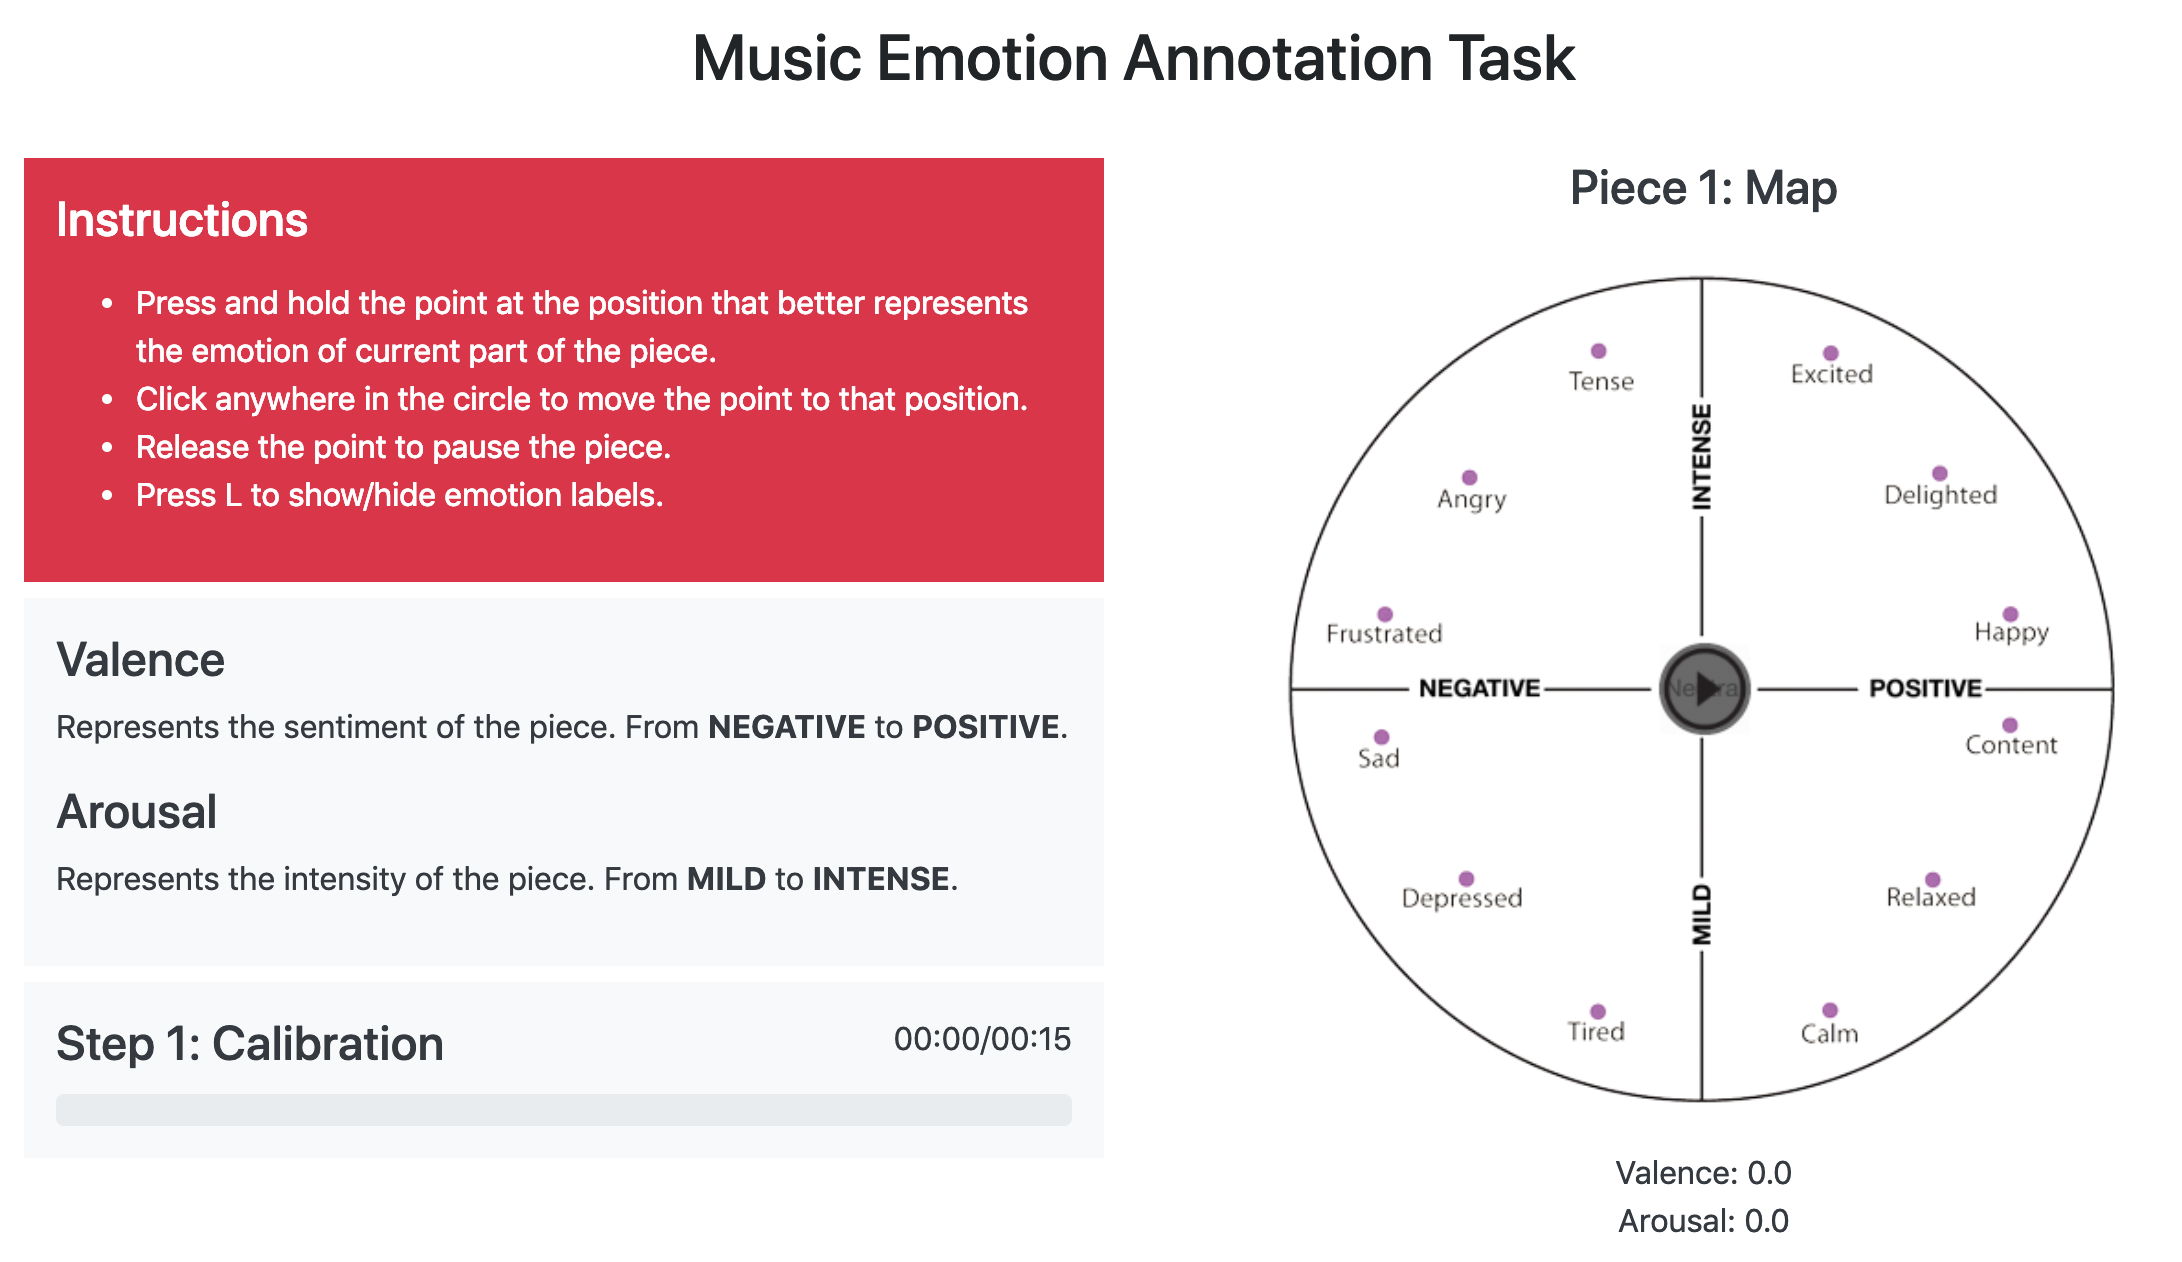
\includegraphics[width=\columnwidth]{imgs/ismir19/annotation_tool.png}
 \caption{Screenshot of the annotation tool.}
 \label{fig:annotation_main}
\end{figure}

\subsection{Data Analysis}
\label{sec:data_analysys}

The annotation task was performed by 1425 annotators, where 55\% are cis female and 42\% are cis male. The other 3\% considered themselves as transgender female, transgender male, genderqueer, or choose not to disclose their gender. All annotators are from the United States and have an average age of approximately 31 years. Musicianship experience was assessed using a 5-point Likert scale where 1 means ``I've never studied music theory or practice'' and 5 means ``I have an undergraduate degree in music''. The average musicianship experience is 2.28. The participants spent on average 12 minutes and 6 seconds to annotate the two pieces.

The data collection process provides a time series of v-a values for each piece. However, only the valence dimension is needed to create a music sentiment dataset. Thus, each piece has 30 time series of valence values. The annotation of each piece was preprocessed, summarized into one time series, and split into ``phrases'' of the same sentiment. The preprocessing is intended to remove noise caused by subjects performing the task randomly to get the reward as fast as possible. The data was preprocessed by smoothing each annotation with a moving average and clustering all 30 time series into 3 clusters (positive, negative, and noise) according to the dynamic time-warping distance metric.

The cluster with the highest variance is considered noise, and so it is discarded. The cluster with more time series among the two remaining ones is then selected and summarized by the mean of its time series. The mean is split at all the points where the valence changes from positive to negative or vice-versa. This process creates several segments with valence values of the same sign, where segments with negative valence are considered negative phrases and segments with positive valence are positive phrases. Figure \ref{fig:clustering} shows an example of this three-step process performed on a piece. All the phrases that had no notes (i.e. silence phrases) were removed. This process created a total of 966 phrases: 599 positive and 367 negative.

\begin{figure}[!h]
 \centering
 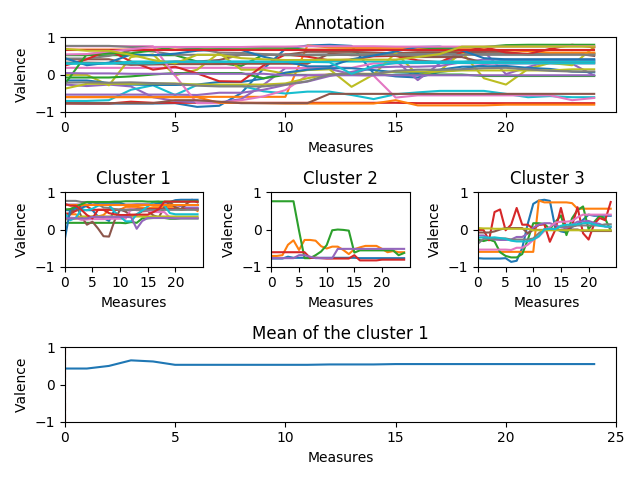
\includegraphics[width=0.9\columnwidth]{imgs/ismir19/clustering.png}
 \caption{Data analysis process used to define the final label of the phrases of a piece. }
 \label{fig:clustering}
\end{figure}


\section{Models and Data Representation}
\label{sec:model}

\citet{radford_2017} used a single-layer multiplicative LSTM (mLSTM) network \cite{krause2017} with 4096 neurons to learn a character-based language model from a sequence of UTF-8 encoded characters. The trained mLSTM was fine-tuned with an extra linear layer to classify sentiment in text. During fine-tuning, the pre-trained weights of the mLSTM were kept frozen, and only the weights of the extra classification layer were trained. Moreover, L1 regularization was used during fine-tuning to enforce a sparse set of weights in the classification layer. This work uses the same models and training procedures to compose music with a target sentiment. Instead of characters, this work represents music pieces as sequences of tokens from a vocabulary representing events retrieved from MIDI files. Sentiment is perceived in music due to several features such as melody, harmony, and tempo \cite{kim2010music}. The proposed representation attempts to encode as many music features\footnote{Constrained by the features one can extract from MIDI data.} as possible while keeping the vocabulary small:

\begin{itemize}
    \item \textbf{n\_[pitch]}: play a note with a given pitch number (any integer from 0 to 127).
    \item \textbf{d\_[duration]\_[dots]}: change the duration of the following notes to a given
    duration with a given amount of dots. Duration types are breve, whole, half, quarter,
    eighth, 16th and 32nd. Dots can be any integer from 0 to 3.
    \item \textbf{v\_[velocity]}: change the velocity of the following  notes to a given velocity (loudness) number. Velocity is discretized in
    bins of size 4, so it can be any integer in the set $V = {4, 8, 12, \dots, 128}$.
    \item \textbf{t\_[tempo]}: change the tempo of the piece to a given tempo in bpm. Tempo is also discretized in bins of size 4, so it can be any integer in the set $T = {24, 28, 32, \dots, 160}$.
    \item \textbf{$\cdot$ (dot)}: end of time step. Each time step is one sixteenth note long.
    \item \textbackslash \textbf{n}: end of piece.
\end{itemize}

For example, Figure \ref{fig:enc_ex} shows the encoding of the first two time steps of the first measure of the \textit{Prelude of Light} from the \textit{Legend of Zelda - Ocarina of Time} . The first time step sets the tempo to 120bpm, the velocity of the following notes to 76, and plays the D Major Triad for the duration of a whole note. The second time step sets the velocity to 84 and plays a dotted quarter A5 note. The total size of this vocabulary is 225, and it represents both the composition and performance elements of a piece (timing and dynamics).

\begin{figure}[!h]
 \centering
 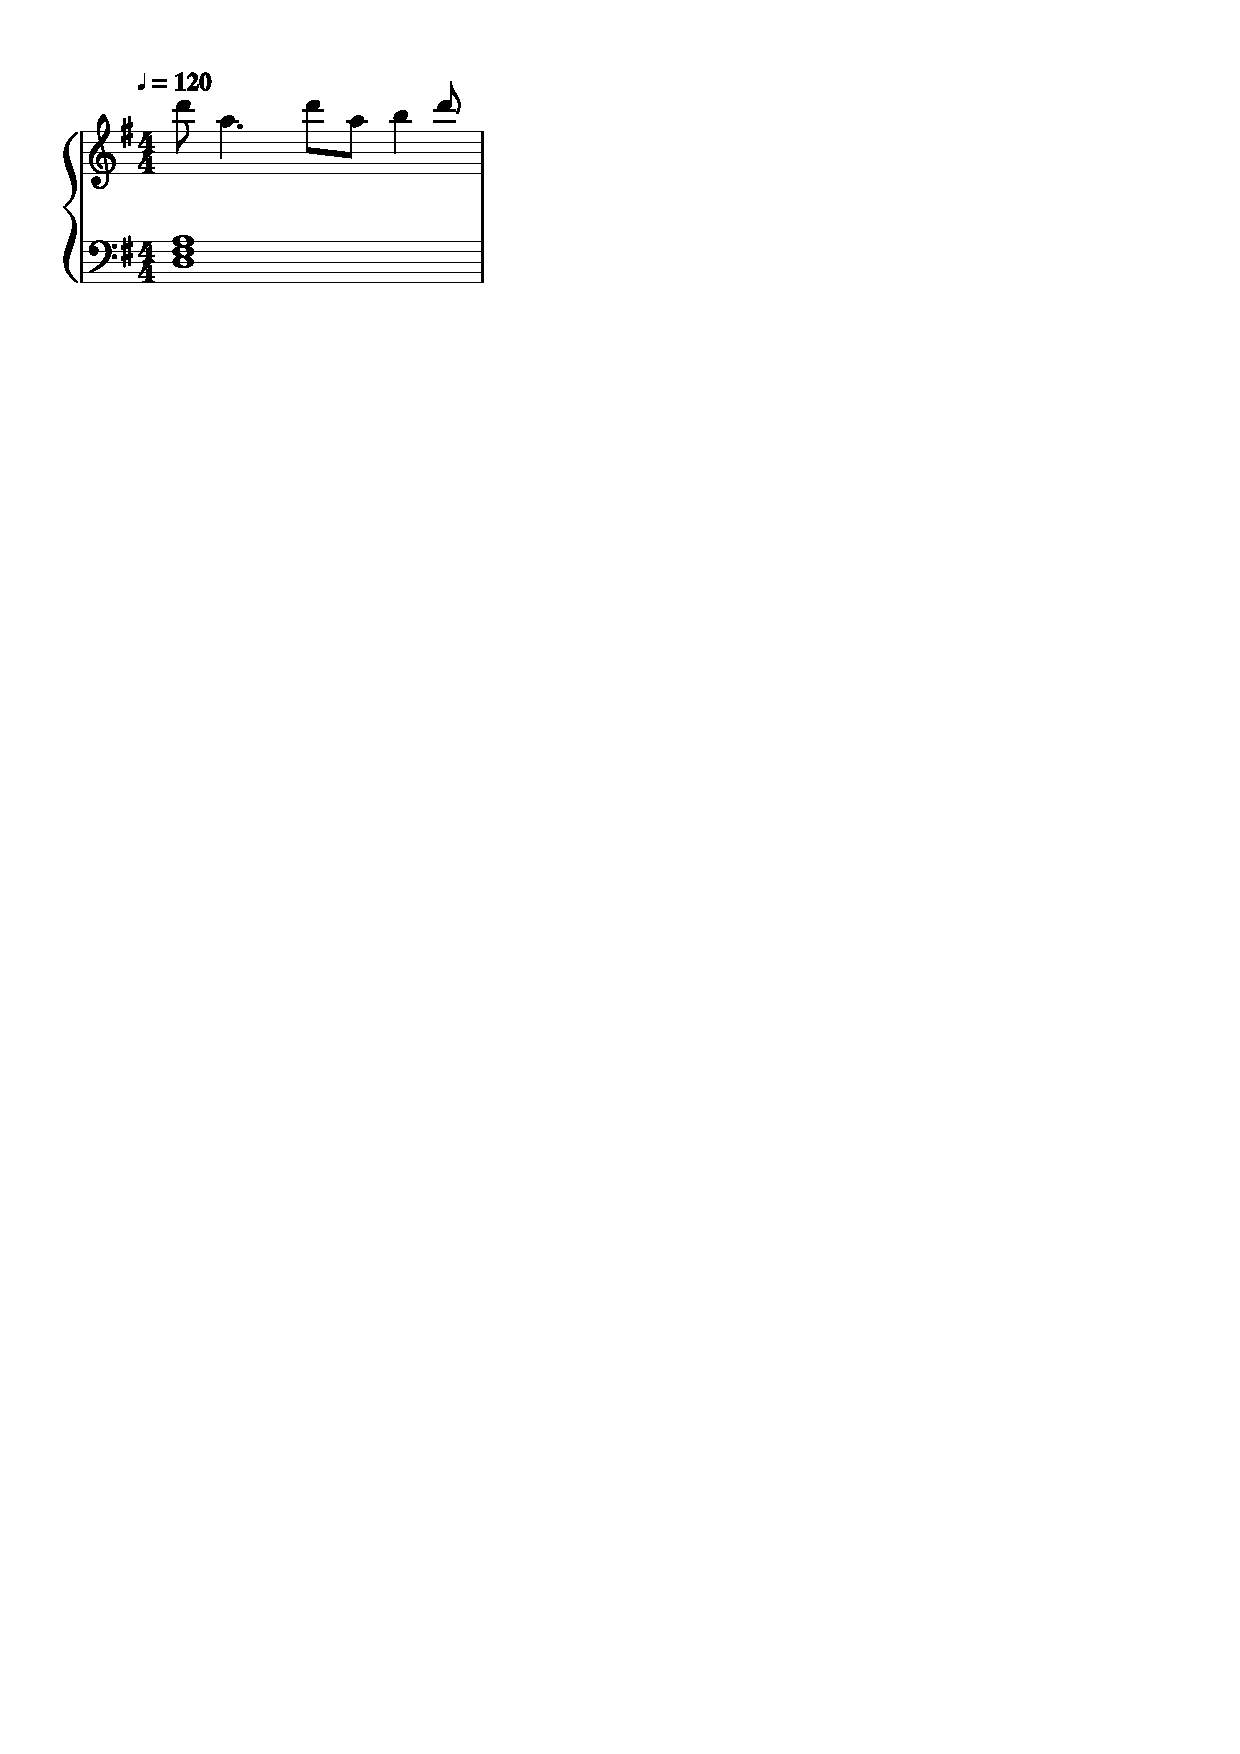
\includegraphics[width=.9\columnwidth]{imgs/ismir19/encoding.pdf}
\begin{spverbatim}
        t_120 v_76 d_whole_0 n_50 n_54 n_57 v_92 d_eighth n_86 . . v_84
        d_quarter_1 n_81 . .
\end{spverbatim}

 \caption{A short example piece encoded using the proposed representation. The encoding represents the first two time steps of the shown measure.}
 \label{fig:enc_ex}
\end{figure}

\section{Sentiment Analysis Evaluation}

The fine-tuning approach proposed in this work is initially evaluated in the sentiment classification task. First, an mLSTM $L$ is pre-trained as a LM with the unlabeled pieces of the VGMIDI dataset. Then, the pre-trained weights of $L$ are frozen, and an additional linear layer $C_f$ is stacked on top of $L$. The resulting model $L + C_f$ is trained as a sentiment classifier with the labeled pieces of the VGMIDI dataset. The final model $L + C_f$ is compared against a baseline mLSTM $C_s$ trained directly on the supervised sentiment classification task. In other words, $C_s$ is trained as a sentiment classifier only with the labeled MIDI phrases (no pre-training involved).

The unlabeled pieces used to train $L$ are augmented in order to create additional training examples, following the methodology of Oore et al. \cite{oore2017learning}. The augmentation consists of time stretching (making each piece up to 5\% faster or slower) and transposition (raising or lowering the pitch of each piece by up to a major third). All these pieces and transformations are encoded according to the proposed word-based representation (see Section \ref{sec:model}). Finally, the encoded pieces are shuffled, and 90\% of them are used for training and 10\% for testing. The training set is divided into three shards of similar size (approximately 18,500 pieces each -- 325MB), and the testing set is combined into one shard (approximately 5800 pieces -- 95MB).

Six different sizes (number of neurons in the hidden layer) are compared for $L$: 128, 256, 512, 1024, 2048, and 4096. For each size, $L$ is trained for 4 epochs using the 3 training shards. Weights are updated with the Adam optimizer after processing sequences of 256 words on mini-batches of size 32. The hidden and cell states of $L$ are initialized to zero at the beginning of each shard. They are also persisted across updates to simulate full-backpropagation and allow for the forward propagation of information outside of a given sequence \cite{radford_2017}. Each sequence is processed by an embedding layer (which is trained together with the mLSTM layer) with 64 neurons before passing through the mLSTM layer. The learning rate is initialized to $5*10^6$ and decayed linearly (after each epoch) to zero over the course of training.

Each $L$ variation is evaluated with a forward pass on the test shard using mini-batches of size 32. Table \ref{tab:gen_anal} shows the average\footnote{Each mini-batch reports one loss.} cross entropy loss for each variation of $L$. The average cross entropy loss decreases as the size of $L$ increases, reaching the best result (loss 1.11) when the size is equal to 4096. Thus, the variation with 4096 neurons is used to proceed with the sentiment classification experiments.

\begin{table}[!h]
 \begin{center}
 \begin{tabular}{cc}
  \hline
  \textbf{mLSTM Size} & \textbf{Average Cross Entropy Loss}\\ \hline
  128 & 1.80   \\
  256  & 1.61  \\
  512  & 1.41  \\
  1024 & 1.25  \\
  2048 & 1.15  \\
  4096 & 1.11  \\ \hline
 \end{tabular}
\end{center}
\caption{Average cross entropy loss of the mLSTM LM with different size (number of neurons in the hidden layer).}
 \label{tab:gen_anal}
\end{table}

After training $L$, an extra linear sentiment classification layer $C_f$ is stacked on top of $L$ and trained on the 966 labeled phrases of the VGMIDI dataset. Here, stacking means passing the final cell state of $L$ as input to $C_f$. During this fine-tuning step, the base layers of $L$ are frozen, which means only the weights of $C_f$ are updated. Moreover, $C_f$ is trained with L1 regularization to shrink the least important of the 4096 feature weights to zero. This ends up highlighting the neurons in $L$ that contain most of the sentiment signal.

The fine-tuning approach $L + C_f$ was compared against the baseline supervised mLSTM $C_s$, which is an mLSTM with exactly the same architecture and size as $L + C_f$ but trained in a fully supervised way. This supervised mLSTM was trained with the same word-based representation of the phrases, but they were padded with silence (the symbol ``.'') in order to equalize their length. Training parameters were set to be the same used to train the base LM. Both methods were evaluated using a 10-fold cross-validation approach, where the test folds have no phrases that appear in the training folds. Table \ref{tab:sent_anal} shows the sentiment classification accuracy of both approaches.

\begin{table}[!h]
 \begin{center}
 \begin{tabular}{lc}
  \hline
  \textbf{Method} & \textbf{Test Accuracy} \\ \hline
  Fine-tuned mLSTM-4096 & 89.83 $\pm$ 3.14\\
  Baseline  mLSTM-4096 & 60.35 $\pm$ 3.52 \\
  \hline
 \end{tabular}
\end{center}
\caption{Average (10-fold cross validation) sentiment classification accuracy of both generative (with logistic regression) and supervised mLSTMs.}
 \label{tab:sent_anal}
\end{table}

The fine-tuned mLSTM achieved an accuracy of 89.83\%, outperforming the supervised mLSTM by 29.48\%. The supervised mLSTM accuracy of 60.35\% suggests that the amount of labeled data (966 phrases) was not enough to learn a good mapping between phrases and sentiment. The accuracy of the fine-tuned mLSTM shows that it is capable of learning, in an unsupervised way, a good representation of sentiment in symbolic music. This is an important result for two reasons. First, since the higher accuracy of fine-tuned mLSTM is derived from unlabeled data, it will be easier to improve this over time using additional (less expensive) unlabeled data instead of the supervised mLSTM approach, which requires additional (expensive) labeled data. Second, because the mLSTM LM was trained to predict the next word in a sequence, it can be used as a music generator. Since it is combined with a sentiment predictor, it opens up the possibility of generating music consistent with a desired sentiment. This idea is explored in the following section.

\section{Generative Evaluation}

To control the sentiment of the music generated by the fine-tuned mLSTM, one has to find the subset of neurons that contain the sentiment signal by exploring the weights of the linear sentiment classification layer. As shown in Figure \ref{fig:final_weights}, the linear classification layer trained with L1 regularization uses 161 neurons out of 4096. Unlike the results of Radford et al. \cite{radford_2017}, the fine-tuning step did not store the sentimental in a single neuron. Instead, the sentiment signal was stored across many neurons in a more balanced way. Therefore, one cannot simply change the values of one neuron to control the sentiment of the output music.

\begin{figure}[!h]
 \centering
 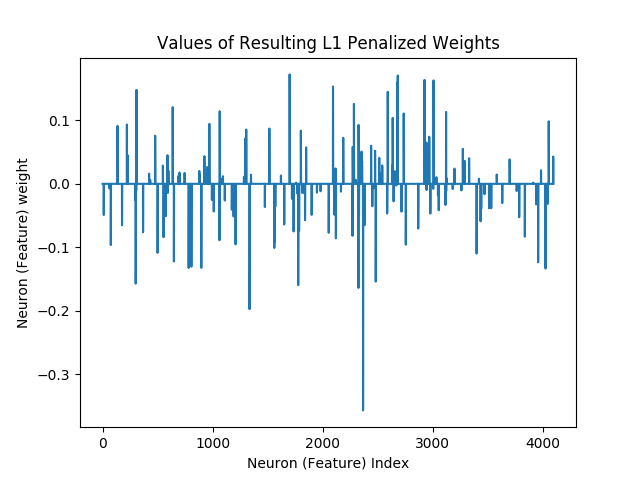
\includegraphics[width=\columnwidth]{imgs/ismir19/weights.png}
 \caption{Weights of 161 L1 neurons. Note multiple prominent positive and negative neurons.}
 \label{fig:final_weights}
\end{figure}

A Genetic Algorithm (GA) was used to optimize the 161 L1 neurons' weights to lead the fine-tuned mLSTM to generate only positive or negative pieces. Each individual in the population of this GA has $161$ real-valued genes representing a small noise to be added to the weights of the $161$ L1 neurons. The fitness of an individual is computed by (i) adding the genes of the individual to the weights (vector addition) of the $161$ L1 neurons of the generative mLSTM, (ii) generating $P$ pieces with this mLSTM, (iii) using the logistic regression model to predict these $P$ generated pieces and (iv) calculating the mean squared error of the $P$ predictions given a target sentiment $s \in S = \{0, 1\}$.

The GA starts with a random population of size 100 where each gene of each individual is a uniformly sampled random number $-2 \leq r \leq 2$. For each generation, the GA (i) evaluates the current population, (ii) selects 100 parents via a roulette wheel with elitism, (iii) recombines the parents (crossover) taking the average of their genes, and (iv) mutates each new recombined individual (new offspring) by randomly setting each gene to a uniformly sampled random number $-2 \leq r \leq 2$.

This GA was executed twice: once to optimize the fine-tuned mLSTM for generating positive pieces and once for negative pieces. Each execution optimized the individuals during 100 epochs with a crossover rate of 95\% and mutation rate of 10\%. To calculate each individual's fitness, $P$=30 pieces were generated with 256 words each, starting with the symbol ``.'' (end of time step). The optimization for positive and negative generation resulted in best individuals with fitness $0.16$ and $0.33$, respectively. This means that if one adds the genes of the best individual of the final population to the weights of the generative mLSTM, one generates positive pieces with 84\% accuracy and negative pieces with 67\% accuracy.

After these two optimization processes, the genes of the best final individual of the positive optimization were added to the weights of the 161 L1 neurons of the trained LM. A set of 30 pieces was then generated with 1000 words starting with the symbol ``.'' (end of time step) and 3 of them were randomly selected. The same process was repeated using the genes of the best final individual of the negative execution. Annotators were asked to label these 6 generated pieces via Amazon MTurk, using the same methodology described in Section \ref{sec:data_collection}. Figure \ref{fig:generated_eval} shows the average valence per measure of each of the generated pieces.

\begin{figure}[!h]
 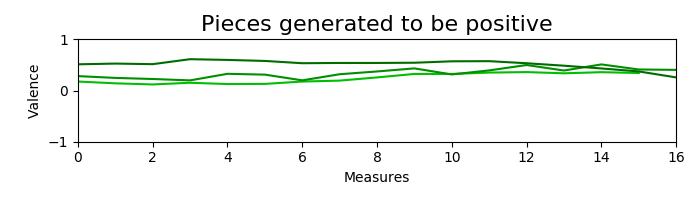
\includegraphics[width=\columnwidth]{imgs/ismir19/means_pos.png}
 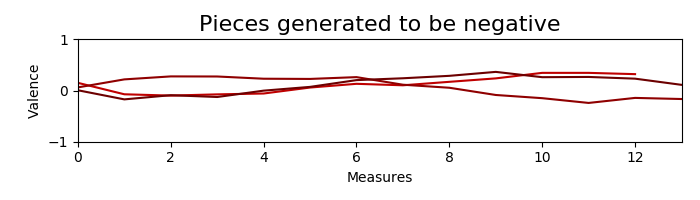
\includegraphics[width=\columnwidth]{imgs/ismir19/means_neg.png}
 \caption{Average valence of the 6 generated pieces, as determined by human annotators.
 %Note that the averages are calculated after clustering the annotations and selecting the cluster
 with least variance.}
 \label{fig:generated_eval}
\end{figure}

These results showed that human annotators agreed that the three positive generated pieces are indeed positive. The generated negative pieces are more ambiguous, having both negative and positive measures. However, as a whole, the negative pieces have lower valence than the positive ones. This suggests that the best negative individual (with fitness $0.33$) encountered by the GA was not good enough to control the mLSTM to generate complete negative pieces. Moreover, the challenge to optimize the L1 neurons suggests that there are more positive pieces than negative ones in the 3 shards used to train the generative mLSTM.

\section{Conclusions}

This chapter presented a mLSTM LM that can be controlled to generate symbolic music with a given sentiment. The mLSTM is controlled with a genetic algorithm that optimizes the weights of specific neurons that are responsible for the sentiment signal. Such neurons are found by fine-tuning the mLSTM with an extra linear layer to classify the sentiment of symbolic music. This fine-tuning approach was evaluated both as a generator and as a sentiment classifier. Results showed that the fine-tuned mLSTM obtained good classification accuracy, outperforming an equivalent mLSTM trained in a fully supervised way. Moreover, a user study showed that humans agree that the fine-tuned LM can generate positive and negative music, with the caveat that the negative pieces are more ambiguous than the positive ones.

% The next chapter presents another search-based approach to control emotion (not only sentiment) in music generated by a LM. This new method was applied to compose background music in real-time for tabletop role-playing games\cite{padovani2017bardo}.
